%--------------------------------------------------------------------
%导言区
% !Mode:: "TeX:UTF-8"

\documentclass[a4paper,UTF8]{ctexrep}
\let\cleardoublepage\clearpage

\usepackage{scuthesis}				% 封面版式
\usepackage{amssymb}  				% 设置数学公式
\usepackage{amsmath} 				% 设置数学公式编号
\usepackage{amsthm}					% 定理
\usepackage{booktabs}

%\usepackage[all,cmtip]{xy}			% xy-pic	画交换图
\usepackage{tikz}			        % tikz      绘图宏包
\usepackage{float}	  				% float		为固定图片位置宏包
\usepackage{subfigure}				% subfigure 引入宏包来添加多张图片 
\usepackage{caption}				% caption   为更改图片命名的宏包
\usepackage{enumerate}				% enumerate 有序列表环境

%\usepackage{boondox-cal}			% boondox-cal   数学花体
%\usepackage{bm}       				% bm 			希腊字母加粗(普通字母类同)

\theoremstyle{plain}
	\newtheorem{thm}{定理~}[chapter]
	\newtheorem{lem}[thm]{引理~}
	\newtheorem{prop}[thm]{命题~}
	\newtheorem{cor}[thm]{推论~}
\theoremstyle{definition}
	\newtheorem{defn}[thm]{定义~}
	\newtheorem{conj}[thm]{猜想~}
	\newtheorem{exmp}[thm]{例~}
	\newtheorem{ques}[thm]{问题~}
	\newtheorem{rem}[thm]{注~}

%	该命令指定公式编号的格式
\numberwithin{equation}{chapter}
\renewcommand{\theequation}{\thechapter.\roman{equation}}

% 请在此处添加或修改你想要的定理样式,以下为英文定理样式,若使用中文写作请注释以下部分,并改用上面的中文定理样式(注意,使用英文写作时,若完成该操作后仍有部分单词显示为中文,请参照ctex文档第6节的“文档汉化”部分自行调整):
% \theoremstyle{plain}
%   \newtheorem{thm}{Theorem}[chapter]
%   \newtheorem{lem}[thm]{Lemma}
%   \newtheorem{prop}[thm]{Proposition}
%   \newtheorem{cor}[thm]{Corollary}
% \theoremstyle{definition}
%   \newtheorem{defn}[thm]{Definition}
%   \newtheorem{conj}[thm]{Conjecture}
%   \newtheorem{exmp}[thm]{Example}
%   \newtheorem{ques}[thm]{Question}
%   \newtheorem{rem}[thm]{Remark}
% \ctexset{bibname = {References}}
% \ctexset{proofname = {Proof}}
% \ctexset{contentsname = {Contents}}

%------------------------------------------------
	%基本信息
	\title{冷空气-蒸汽对流传热实验报告}
	\titleEng{Experimental Report of Cold air-steam convection heat transfer}
	
	\author{王诗煜}
	\authorEng{Shiyu Wang}
	\adviser{吴潘}
	\adviserEng{Pan Wu}
	
	\college{化学工程学院}
	\collegeEng{School of Chemical Engineering}
	\major{化学工程与工艺(虚拟的)}
	\majorEng{Chemical Engineering and Technics(virtual)}
	
	\grade{2023}
	\id{2022141500089}
	\date{\today}
	
 			% 作者信息


%-----------------------------------------------------------------
%正文区
	\begin{document}
	\zihao{-4}
	
	% 封面+摘要
	\makecover

\begin{abstract}{化工原理实验; 流体力学}
这一部分有意留白。
\end{abstract}


\begin{abstractEng}{Chemical Engineering Experiment; Fluid Mechaics}
This part intentionally left black.
\end{abstractEng}


\tableofcontents

        \chapter{报告正文}
	% 正文
	\section{实验目的}
	%----------------------------------------------
	\begin{enumerate}
		\item 掌握流体流经直管和管件时阻力损失的测定方法,了解流体流动中能量损失的变化规律。
            
            \item 测定流体在直管内流动时的直管阻力,绘制摩擦系数$\lambda$与雷诺数$Re$的关系曲线。
            \item 测定一定转速下离心泵的特性曲线。
            \item 了解离心泵结构,学会离心泵的操作和流量调节的方法。
            \item 测定单台离心泵运行时的管路特性曲线。
            \item 标定孔板流量计,绘制流量系数$C_0$与雷诺数$Re$的关系曲线。
            \item 熟悉流量、压差和温度等的化工仪表的使用。
	\end{enumerate}

        \section{实验原理}
        \subsection{测定雷诺数与$\lambda$关系曲线}
        流体在流动时的机械能包括动能、位能和静压能,实际流体在管内流动过程中有一部分机械能因摩擦而转化为热能,导致动能损失,因此各截面上机械能是不相等的,两截面的机械能之差是流体在两截面之间转换为热能的机械能,这部分机械能称为流体的阻力损失。

对单位质量流体为衡算基准,在1-1截面、2-2截面之间稳定流动且无外加功时,伯努利方程如下:
\begin{equation}
    gz_1+\frac{p_1}{\rho}+\frac{u_1^2}{2}=gz_2+\frac{p_2}{\rho}+\frac{u_2^2}{2}+\Sigma h_f
\end{equation}
其中,$z_1$和$z_2$分别位两截面的高度,$p_1$和$p_2$为两截面处流体的静压,$\rho$为流体密度,$\Sigma h_f$为流体在两截面间的总阻力损失。

实验时,使1-1和2-2截面的管道截面积相等,从而两截面的流速相等,这样以来只要测出两截面的位差以及静压差即可根据伯努利方程算出阻力损失。

当流体通过水平管时,阻力损失如下:
\begin{equation}
    h_f = \frac{p_1 - p_2}{\rho}= \frac{\Delta p}{\rho}
\end{equation}

直管阻力损失的计算公式为:
\begin{equation}
    h_f = \lambda \cdot \frac{l}{d} \cdot \frac{u_2^2}{2} 
\end{equation}

由(1.ii)与(1.iii)两式联立得:
\begin{equation}
    \lambda = \frac{\Delta p}{\rho}\cdot \frac{d}{l} \cdot \frac{2}{u^2}
\end{equation}

而雷诺数的计算公式为:
\begin{equation}
    Re = \frac{du\rho}{\mu}
\end{equation}

管径和管长可以直接测量得到,流速可以通过测流量间接测出,压差通过差压变送器测出,从而我们可以测出流体的阻力损失,雷诺数与$\lambda$,通过调节离心泵出口阀开度,我们便可测得不同流速下的雷诺数与$\lambda$,从而可以绘制出雷诺数与$\lambda$的关系曲线。
\subsection{测定离心泵特性曲线}
离心泵的性能参数有流量$q_v$、扬程(压头)$H$、轴功率$N$、效率$\eta$和允许汽蚀余量或吸上真空高度等。泵在一定转速下,扬程、轴功率、效率均随流量的变化而变化,通常将扬程与流量、功率与流量、效率与流量三条曲线称为离心泵的特性曲线。离心泵的特性曲线是选择和使用离心泵的重要依据。

本实验需要测量出流量, 扬程, 轴功率, 效率这四个性能参数. 其中流量可以直接用电磁流量计测得, 其它三个性能参数则需要计算. 

扬程的计算方法: 在泵的入口与出口列伯努利方程:
\begin{equation}
    H=\frac{p_2-p_1}{\rho g}+\Delta Z + \frac{u^2_2-u^2_1}{2g}+\Sigma H_{f1-2}
\end{equation}

因为进出口管径相等, 所以对应流速相等, 并且泵内阻力损失约等于0,所以上式变为:

\begin{equation}
    H=\frac{p_2-p_1}{\rho g}+\Delta Z
\end{equation}

因此只要测出进出口高度差和压力差即可算出离心泵扬程.

离心泵电功率与轴功率的关系为轴功率等于电功率乘以传动效率与与电机效率的乘积:
\begin{equation}
    N=N_{elect} \times \eta_{elect} \times \eta_{trans}
\end{equation}
这里传动效率与电机效率的乘积近似取为0.95, 之后就可以由电功率计算轴功率了.

计算出扬程之后就可以由扬程计算有效功率, 再将有效功率与轴功率相除就是离心泵的效率了.
\begin{equation}
    \eta =\frac{N_e}{N}\times 100\%= \frac{q_v H \rho g}{N}\times 100\%
\end{equation}

效率的最高点称为设计点。离心泵在此点对应的流量和扬程下工作最为经济,因此与高效率点对应的参数称为最佳工况参数。一般将最高效率值的92\%的范围称为泵的高效区,泵应尽量在该范围内操作。

\subsection{标定孔板流量计}
当流体流经孔板流量计的锐孔时,流通截面突然收缩,流体流经孔板时因流道缩小、流浦增大,即动能增大,且由于惯性作用从孔口流出后继续收缩形成最小截面(称为缩脉),缩脉处流速最大因而静压相应最低,在孔板前上游截面和此缩脉截面之间列伯努利方程式,通过连续性方程整理得:
\begin{equation}
    u_0=C_0\sqrt{\frac{2(p_1-p_2)}{\rho}}
\end{equation}
\begin{equation}
    q_v=A_0u_0=C_0A_0\sqrt{\frac{2(p_1-p_2)}{\rho}}
\end{equation}

其中$A_0$是孔口的横截面积,因此只要知道孔口直径并测得流体流速与压差就可以算出孔流系数, 再按照定义算出此时的雷诺数即可绘制雷诺数与孔流系数的关系曲线. 




        \section{实验装置图及主要设备(包括名称、型号、规格)}
实验装置图如下:


\begin{figure}[h]
    \centering
    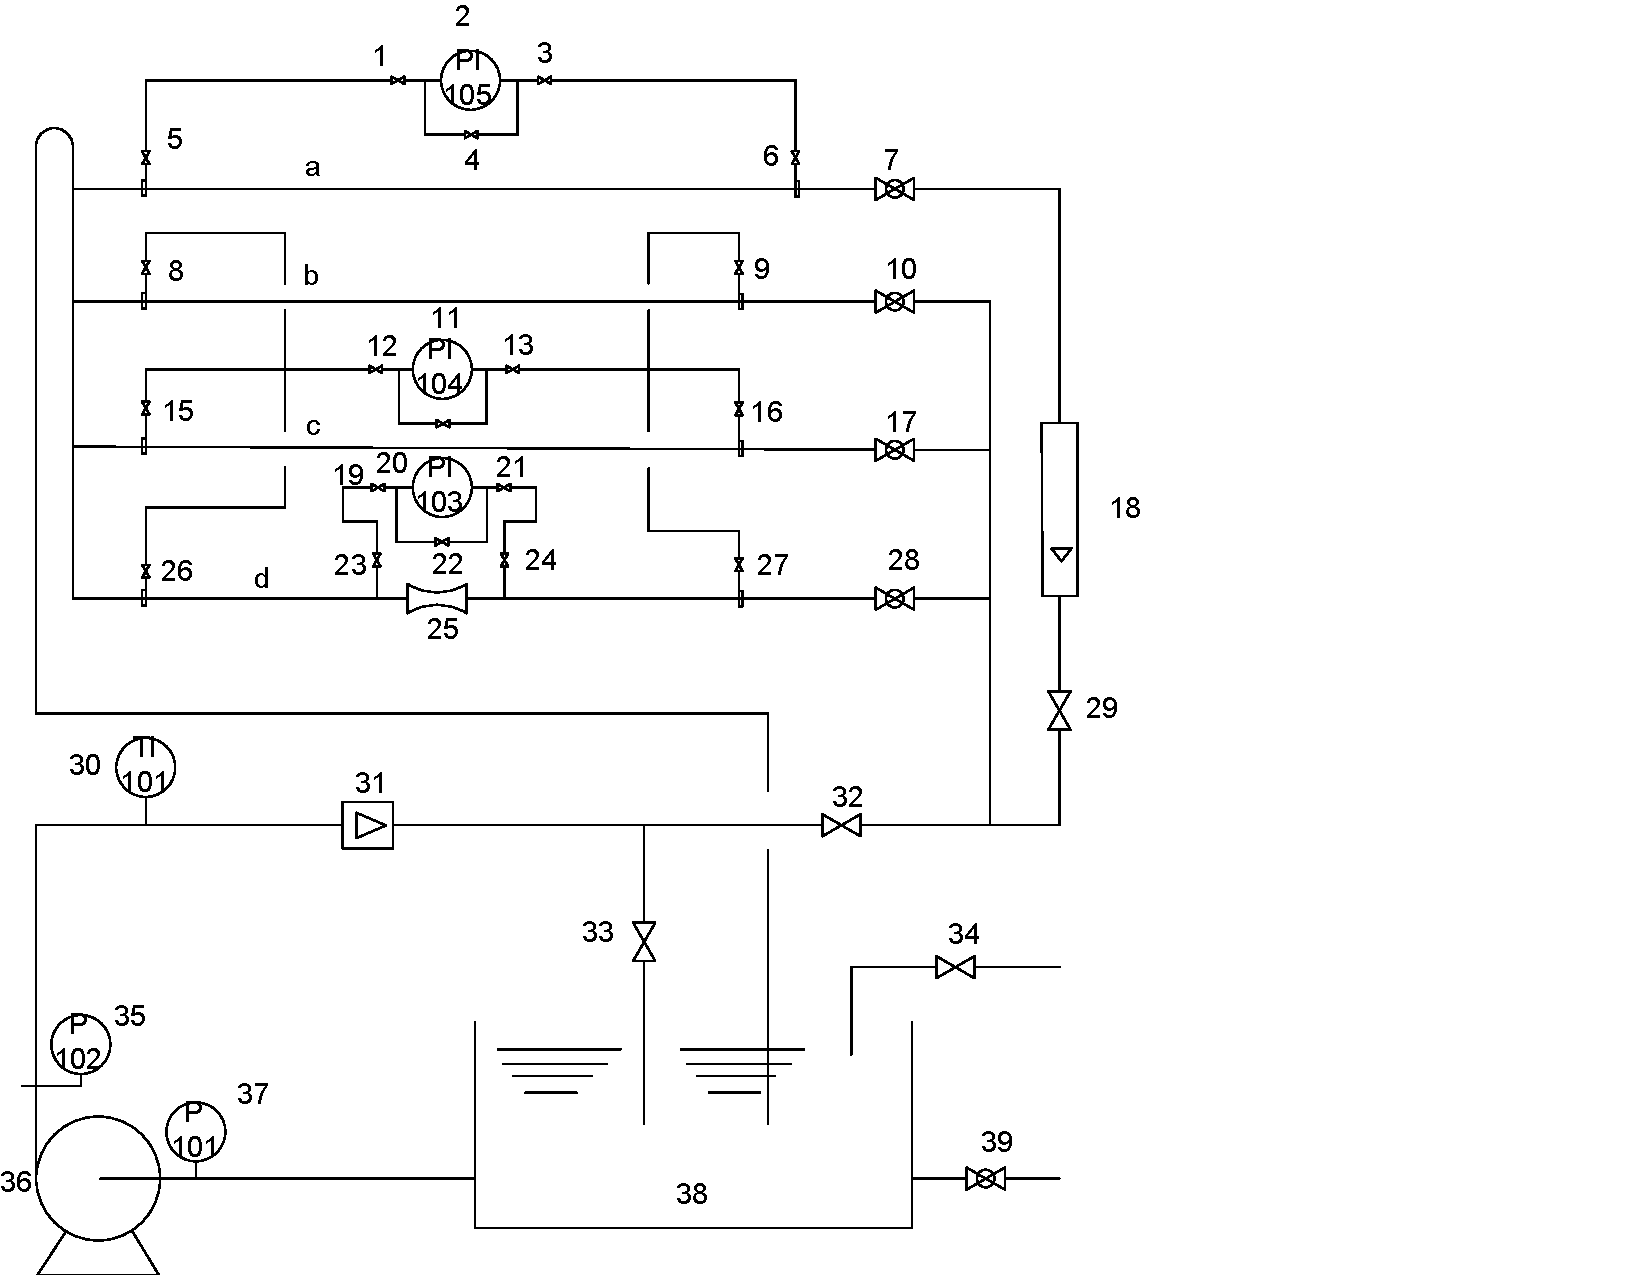
\includegraphics[width=0.7\linewidth]{流体力学实验装置示意图.pdf}
    \caption{本实验的装置示意图}
    \label{fig:enter-label}
\end{figure}

    实验所使用的设备如下:
    
    
\begin{itemize}
    \item 内径为27mm的钢管与铜管
    \item 内径为6mm的钢管
    \item 与管径相匹配的球阀与闸阀
    \item 特性曲线未知的离心泵
    \item 孔径为19.5mm的孔板流量计, 量程合适的电磁流量计与转子流量计以及差压变送器
    \item 变频器, 功率表与转速表
\end{itemize}


        \section{实验步骤}

        \begin{enumerate}
            \item 关闭离心泵出口阀与所有分支管路的阀门,打开所有测压三通阀, 开启总电源与仪表电源.
            \item 检查并保持离心泵的进口管路畅通,确保流体已充满离心泵,启动离心泵,设定电机频率为25$hz$。离心泵启动后,如果声音异常,应及时关闭离心泵进行检查.
            \item 开启b管路的球阀10, 再全开闸阀32, 排除所测管路中的空气.
            \item 关闭所测管路对应差压变送器的测压三通阀, 稳定2分钟后记录流量和压差数据, 适当关小闸阀32,稳定后再进行记录,重复这一过程在流量大于1立方米每时的情况下记录12组数据.
            \item 用同样的方法完成c管路的测量.
            \item 接着测量a管路, 此时通过锥形阀29调节流量, 测量12组数据并保证至少4组为层流, 完成阻力损失的测量.
            \item 接着关闭闸阀32以及所有分支管路的球阀开启所有测压三通阀, 全开闸阀33, 调节流量从最大到零, 每调节一次之后稳定2分钟再读取离心泵进出口压力, 管路中的流速以及离心泵总功率, 共测量至少12组数据. 
            \item 之后进行孔板流量计的标定, 开启球阀28, 关闭闸阀33并全开闸阀32, 排除管内空气后关闭对应的测压三通阀, 通过闸阀32调节流量, 在流量从最大到1立方米每时之间测量10组压差和流量数据, 每两次测量之间稳定2分钟
            \item 实验结束, 关闭闸阀32和球阀28,变频调零,依次关闭离心泵电源、仪表电源和总电源。
        \end{enumerate}
\newpage
        \section{实验原始数据记录列表}
\begin{figure}[h]
    \centering
    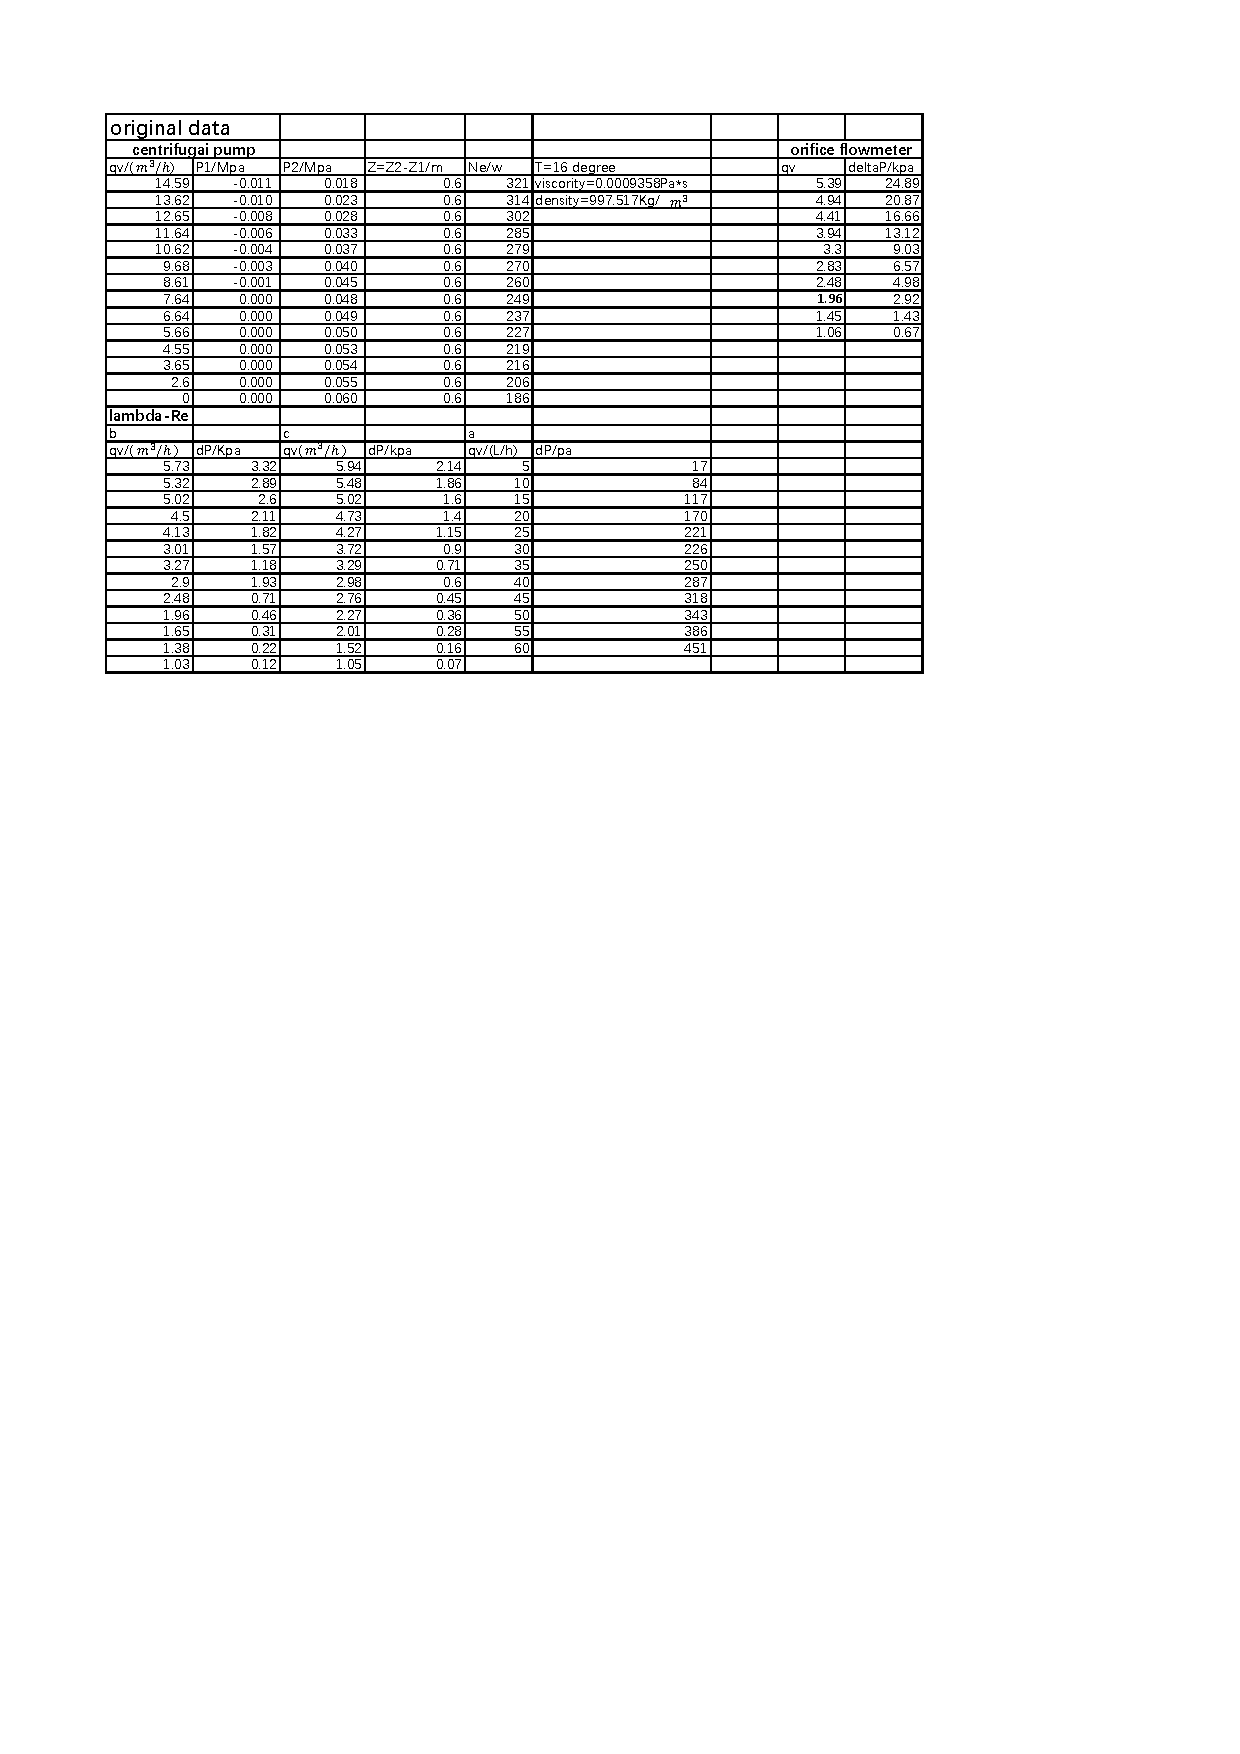
\includegraphics[width=\linewidth]{5th_orig.pdf}
    \caption{本实验的原始数据}
    \label{fig:enter-label}
\end{figure}


        \section{实验数据处理(以一组实验数据为例进行计算)}
        \subsection{$\lambda$ 与 $Re$ 关系曲线实验}
        在这里,我们需要在流量与压差已知的情况下算出$\lambda$和$Re$,这里以第一组数据为例。

        此时,$q_v=5.73m^3/h, \Delta P = 3.32Kpa, d=27mm, l=1430mm$将数据带入公式算出此时流速为:

        $$ u =\frac{q_v}{A^2}=\frac{4q_v}{\pi d^2}=2.78m/s$$

        之后就可以由$Re$的定义以及直管阻力损失的计算式算出$Re$和$\lambda$:
        $$Re= \frac{du\rho}{\mu}=80049 $$
        $$\lambda = \frac{2d\Delta p}{\rho l u^2  }=0.01625$$  

        用同样的方法可以算出其余组的$Re$和$\lambda$
        
        \subsection{离心泵特性曲线}
        在这里,我们需要在流量,离心泵进出口压差和高度差以及输入功率已知的情况下算出扬程,轴功率以及效率。以第一组数据为例:

        此时输入功率为321瓦,取电机效率与传递效率的乘积为0.95,则有:
        $$N=N_{elect} \times \eta_{elect} \times \eta_{trans} = 304.95W $$

        此时进出口管路管径相等,由伯努利方程计算泵的扬程:

        $$H=\frac{p_2-p_1}{\rho g}+\Delta H_2O$$

        之后由扬程算出有效功率,再与轴功率相除算出效率:
        $$\eta = \frac{q_v H \rho g}{N}\times 100\%= 45.68\%$$
        
        
        \subsection{孔板流量计标定}
        这里需要在压差与流量已知的情况下算出孔流系数与雷诺数。以第一组数据为例:
        $$C_0=\frac{u _0}{\sqrt{\frac{2\Delta P}{\rho}}}=\frac{4q_v}{\pi d^2 \sqrt{\frac{2\Delta P}{\rho}}}=0.71$$

        接着再根据雷诺数的定义计算雷诺数:
        $$Re_d= \frac{du\rho}{\mu}= \frac{4q_v\rho}{\pi d\mu}=75300$$
        \newpage
        \section{实验结果、结论与分析}
\subsection{实验结果}
b管的$Re$与$\lambda$关系曲线如下:
\begin{figure}[h]
    \centering
    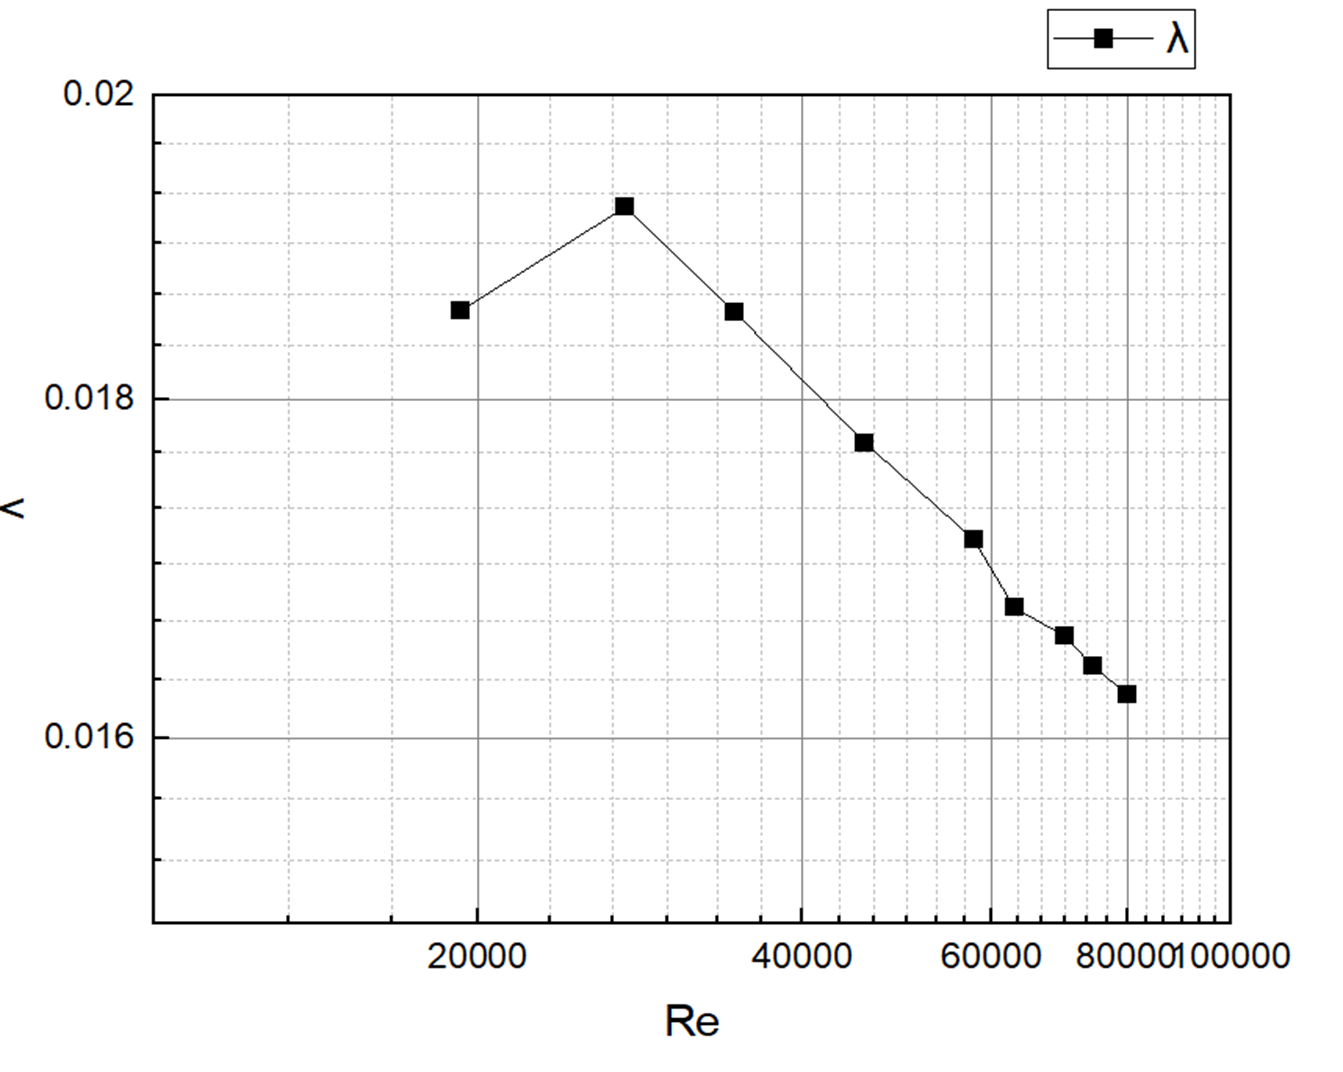
\includegraphics[width=0.6\linewidth]{image.png}
    \caption{b管的$Re$与$\lambda$关系曲线}
    \label{fig:enter-label}
\end{figure}

c管的$Re$与$\lambda$关系曲线如下:
\begin{figure}[h]
    \centering
    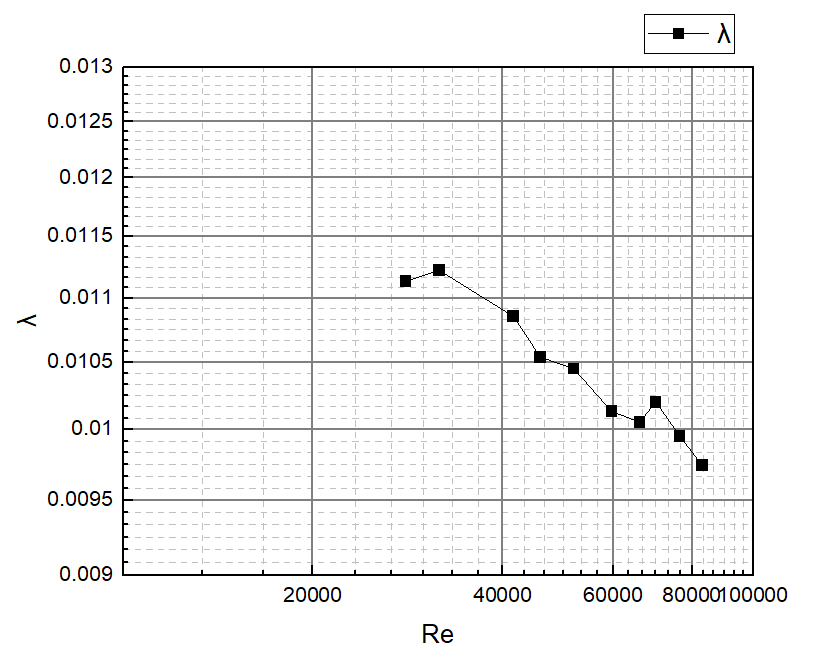
\includegraphics[width=0.6\linewidth]{imagee.png}
    \caption{c管的$Re$与$\lambda$关系曲线}
    \label{fig:enter-label}
\end{figure}
\newpage
a管的$Re$与$\lambda$关系曲线如下:
\begin{figure}[h]
    \centering
    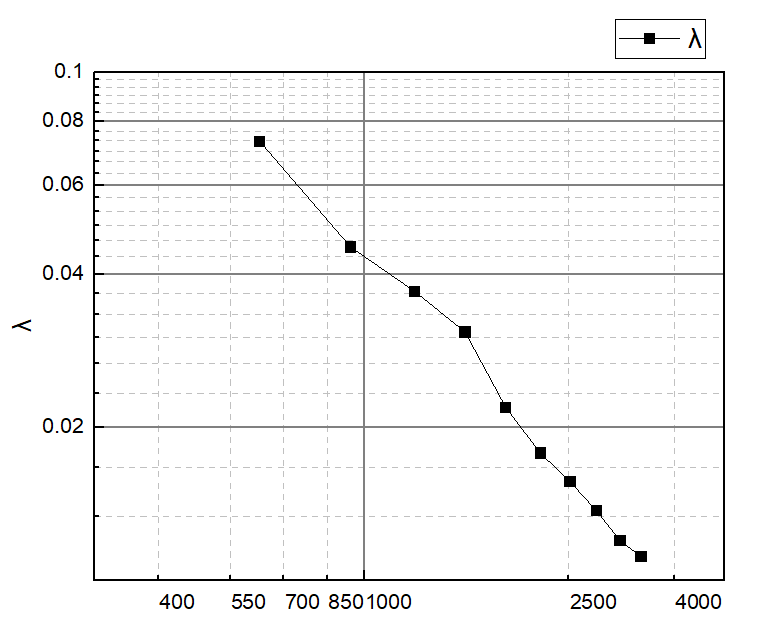
\includegraphics[width=0.7\linewidth]{ihumage.png}
    \caption{a管的$Re$与$\lambda$关系曲线}
    \label{fig:enter-label}
\end{figure}

离心泵特性曲线如下:

\begin{figure}[h]
    \centering
    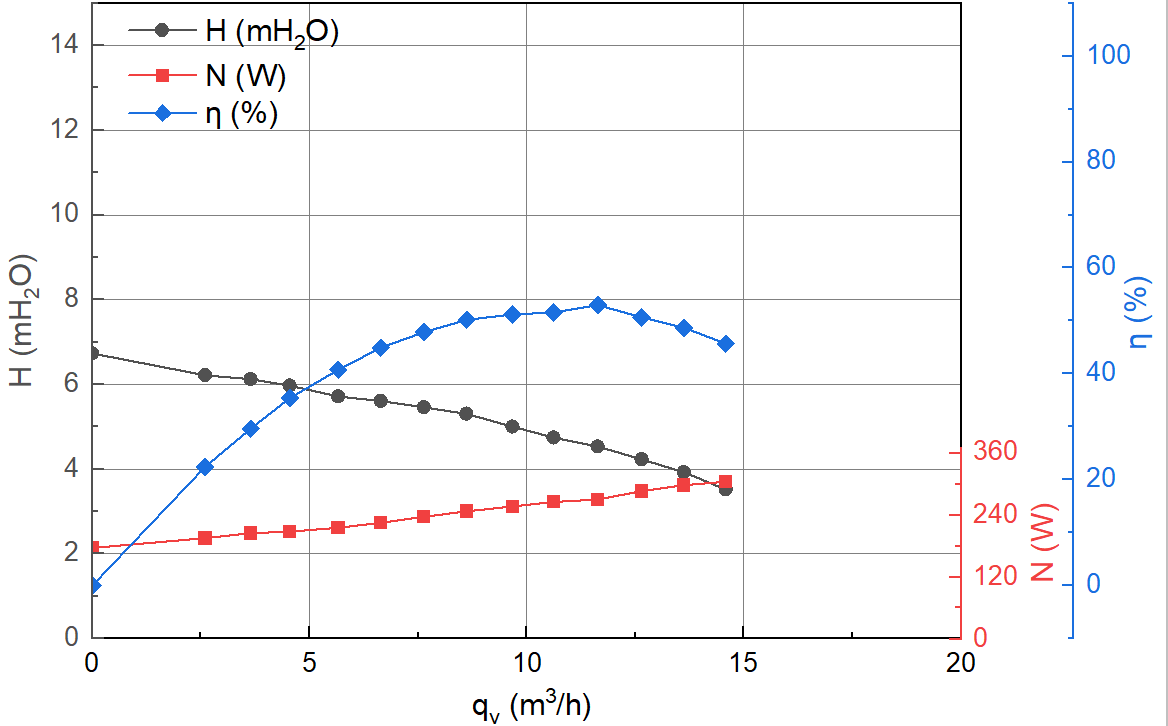
\includegraphics[width=0.7\linewidth]{hio.png}
    \caption{离心泵特性曲线}
    \label{fig:enter-label}
\end{figure}

\begin{tikzpicture}[width=0.7\linewidth]

\def\CheckTikzLibraryLoaded#1{ \ifcsname tikz@library@#1@loaded\endcsname \else \PackageWarning{tikz}{usetikzlibrary{#1} is missing in the preamble.} \fi }
\CheckTikzLibraryLoaded{patterns}
\CheckTikzLibraryLoaded{plotmarks}
\pgfdeclareplotmark{cross} {
\pgfpathmoveto{\pgfpoint{-0.3\pgfplotmarksize}{\pgfplotmarksize}}
\pgfpathlineto{\pgfpoint{+0.3\pgfplotmarksize}{\pgfplotmarksize}}
\pgfpathlineto{\pgfpoint{+0.3\pgfplotmarksize}{0.3\pgfplotmarksize}}
\pgfpathlineto{\pgfpoint{+1\pgfplotmarksize}{0.3\pgfplotmarksize}}
\pgfpathlineto{\pgfpoint{+1\pgfplotmarksize}{-0.3\pgfplotmarksize}}
\pgfpathlineto{\pgfpoint{+0.3\pgfplotmarksize}{-0.3\pgfplotmarksize}}
\pgfpathlineto{\pgfpoint{+0.3\pgfplotmarksize}{-1.\pgfplotmarksize}}
\pgfpathlineto{\pgfpoint{-0.3\pgfplotmarksize}{-1.\pgfplotmarksize}}
\pgfpathlineto{\pgfpoint{-0.3\pgfplotmarksize}{-0.3\pgfplotmarksize}}
\pgfpathlineto{\pgfpoint{-1.\pgfplotmarksize}{-0.3\pgfplotmarksize}}
\pgfpathlineto{\pgfpoint{-1.\pgfplotmarksize}{0.3\pgfplotmarksize}}
\pgfpathlineto{\pgfpoint{-0.3\pgfplotmarksize}{0.3\pgfplotmarksize}}
\pgfpathclose
\pgfusepathqstroke
}
\pgfdeclareplotmark{cross*} {
\pgfpathmoveto{\pgfpoint{-0.3\pgfplotmarksize}{\pgfplotmarksize}}
\pgfpathlineto{\pgfpoint{+0.3\pgfplotmarksize}{\pgfplotmarksize}}
\pgfpathlineto{\pgfpoint{+0.3\pgfplotmarksize}{0.3\pgfplotmarksize}}
\pgfpathlineto{\pgfpoint{+1\pgfplotmarksize}{0.3\pgfplotmarksize}}
\pgfpathlineto{\pgfpoint{+1\pgfplotmarksize}{-0.3\pgfplotmarksize}}
\pgfpathlineto{\pgfpoint{+0.3\pgfplotmarksize}{-0.3\pgfplotmarksize}}
\pgfpathlineto{\pgfpoint{+0.3\pgfplotmarksize}{-1.\pgfplotmarksize}}
\pgfpathlineto{\pgfpoint{-0.3\pgfplotmarksize}{-1.\pgfplotmarksize}}
\pgfpathlineto{\pgfpoint{-0.3\pgfplotmarksize}{-0.3\pgfplotmarksize}}
\pgfpathlineto{\pgfpoint{-1.\pgfplotmarksize}{-0.3\pgfplotmarksize}}
\pgfpathlineto{\pgfpoint{-1.\pgfplotmarksize}{0.3\pgfplotmarksize}}
\pgfpathlineto{\pgfpoint{-0.3\pgfplotmarksize}{0.3\pgfplotmarksize}}
\pgfpathclose
\pgfusepathqfillstroke
}
\pgfdeclareplotmark{newstar} {
\pgfpathmoveto{\pgfqpoint{0pt}{\pgfplotmarksize}}
\pgfpathlineto{\pgfqpointpolar{44}{0.5\pgfplotmarksize}}
\pgfpathlineto{\pgfqpointpolar{18}{\pgfplotmarksize}}
\pgfpathlineto{\pgfqpointpolar{-20}{0.5\pgfplotmarksize}}
\pgfpathlineto{\pgfqpointpolar{-54}{\pgfplotmarksize}}
\pgfpathlineto{\pgfqpointpolar{-90}{0.5\pgfplotmarksize}}
\pgfpathlineto{\pgfqpointpolar{234}{\pgfplotmarksize}}
\pgfpathlineto{\pgfqpointpolar{198}{0.5\pgfplotmarksize}}
\pgfpathlineto{\pgfqpointpolar{162}{\pgfplotmarksize}}
\pgfpathlineto{\pgfqpointpolar{134}{0.5\pgfplotmarksize}}
\pgfpathclose
\pgfusepathqstroke
}
\pgfdeclareplotmark{newstar*} {
\pgfpathmoveto{\pgfqpoint{0pt}{\pgfplotmarksize}}
\pgfpathlineto{\pgfqpointpolar{44}{0.5\pgfplotmarksize}}
\pgfpathlineto{\pgfqpointpolar{18}{\pgfplotmarksize}}
\pgfpathlineto{\pgfqpointpolar{-20}{0.5\pgfplotmarksize}}
\pgfpathlineto{\pgfqpointpolar{-54}{\pgfplotmarksize}}
\pgfpathlineto{\pgfqpointpolar{-90}{0.5\pgfplotmarksize}}
\pgfpathlineto{\pgfqpointpolar{234}{\pgfplotmarksize}}
\pgfpathlineto{\pgfqpointpolar{198}{0.5\pgfplotmarksize}}
\pgfpathlineto{\pgfqpointpolar{162}{\pgfplotmarksize}}
\pgfpathlineto{\pgfqpointpolar{134}{0.5\pgfplotmarksize}}
\pgfpathclose
\pgfusepathqfillstroke
}
\definecolor{c}{rgb}{1,1,1};
\draw [color=c, fill=c] (0,0) rectangle (20,14.411);
\draw [color=c, fill=c] (2,1.4411) rectangle (18,12.9699);
\definecolor{c}{rgb}{0,0,0};
\draw [c,line width=0.9] (2,1.4411) -- (2,12.9699) -- (18,12.9699) -- (18,1.4411) -- (2,1.4411);
\definecolor{c}{rgb}{1,1,1};
\draw [color=c, fill=c] (2,1.4411) rectangle (18,12.9699);
\definecolor{c}{rgb}{0,0,0};
\draw [c,line width=0.9] (2,1.4411) -- (2,12.9699) -- (18,12.9699) -- (18,1.4411) -- (2,1.4411);
\draw [c,line width=0.9] (2,1.4411) -- (18,1.4411);
\draw [c,line width=0.9] (2,1.78697) -- (2,1.4411);
\draw [c,line width=0.9] (2.32323,1.61404) -- (2.32323,1.4411);
\draw [c,line width=0.9] (2.64646,1.61404) -- (2.64646,1.4411);
\draw [c,line width=0.9] (2.9697,1.61404) -- (2.9697,1.4411);
\draw [c,line width=0.9] (3.29293,1.61404) -- (3.29293,1.4411);
\draw [c,line width=0.9] (3.61616,1.78697) -- (3.61616,1.4411);
\draw [c,line width=0.9] (3.93939,1.61404) -- (3.93939,1.4411);
\draw [c,line width=0.9] (4.26263,1.61404) -- (4.26263,1.4411);
\draw [c,line width=0.9] (4.58586,1.61404) -- (4.58586,1.4411);
\draw [c,line width=0.9] (4.90909,1.61404) -- (4.90909,1.4411);
\draw [c,line width=0.9] (5.23232,1.78697) -- (5.23232,1.4411);
\draw [c,line width=0.9] (5.55556,1.61404) -- (5.55556,1.4411);
\draw [c,line width=0.9] (5.87879,1.61404) -- (5.87879,1.4411);
\draw [c,line width=0.9] (6.20202,1.61404) -- (6.20202,1.4411);
\draw [c,line width=0.9] (6.52525,1.61404) -- (6.52525,1.4411);
\draw [c,line width=0.9] (6.84848,1.78697) -- (6.84848,1.4411);
\draw [c,line width=0.9] (7.17172,1.61404) -- (7.17172,1.4411);
\draw [c,line width=0.9] (7.49495,1.61404) -- (7.49495,1.4411);
\draw [c,line width=0.9] (7.81818,1.61404) -- (7.81818,1.4411);
\draw [c,line width=0.9] (8.14141,1.61404) -- (8.14141,1.4411);
\draw [c,line width=0.9] (8.46465,1.78697) -- (8.46465,1.4411);
\draw [c,line width=0.9] (8.78788,1.61404) -- (8.78788,1.4411);
\draw [c,line width=0.9] (9.11111,1.61404) -- (9.11111,1.4411);
\draw [c,line width=0.9] (9.43434,1.61404) -- (9.43434,1.4411);
\draw [c,line width=0.9] (9.75758,1.61404) -- (9.75758,1.4411);
\draw [c,line width=0.9] (10.0808,1.78697) -- (10.0808,1.4411);
\draw [c,line width=0.9] (10.404,1.61404) -- (10.404,1.4411);
\draw [c,line width=0.9] (10.7273,1.61404) -- (10.7273,1.4411);
\draw [c,line width=0.9] (11.0505,1.61404) -- (11.0505,1.4411);
\draw [c,line width=0.9] (11.3737,1.61404) -- (11.3737,1.4411);
\draw [c,line width=0.9] (11.697,1.78697) -- (11.697,1.4411);
\draw [c,line width=0.9] (12.0202,1.61404) -- (12.0202,1.4411);
\draw [c,line width=0.9] (12.3434,1.61404) -- (12.3434,1.4411);
\draw [c,line width=0.9] (12.6667,1.61404) -- (12.6667,1.4411);
\draw [c,line width=0.9] (12.9899,1.61404) -- (12.9899,1.4411);
\draw [c,line width=0.9] (13.3131,1.78697) -- (13.3131,1.4411);
\draw [c,line width=0.9] (13.6364,1.61404) -- (13.6364,1.4411);
\draw [c,line width=0.9] (13.9596,1.61404) -- (13.9596,1.4411);
\draw [c,line width=0.9] (14.2828,1.61404) -- (14.2828,1.4411);
\draw [c,line width=0.9] (14.6061,1.61404) -- (14.6061,1.4411);
\draw [c,line width=0.9] (14.9293,1.78697) -- (14.9293,1.4411);
\draw [c,line width=0.9] (15.2525,1.61404) -- (15.2525,1.4411);
\draw [c,line width=0.9] (15.5758,1.61404) -- (15.5758,1.4411);
\draw [c,line width=0.9] (15.899,1.61404) -- (15.899,1.4411);
\draw [c,line width=0.9] (16.2222,1.61404) -- (16.2222,1.4411);
\draw [c,line width=0.9] (16.5455,1.78697) -- (16.5455,1.4411);
\draw [c,line width=0.9] (16.5455,1.78697) -- (16.5455,1.4411);
\draw [c,line width=0.9] (16.8687,1.61404) -- (16.8687,1.4411);
\draw [c,line width=0.9] (17.1919,1.61404) -- (17.1919,1.4411);
\draw [c,line width=0.9] (17.5152,1.61404) -- (17.5152,1.4411);
\draw [c,line width=0.9] (17.8384,1.61404) -- (17.8384,1.4411);
\draw [anchor=base] (2,0.965539) node[scale=1.11327, color=c, rotate=0]{0};
\draw [anchor=base] (3.61616,0.965539) node[scale=1.11327, color=c, rotate=0]{1};
\draw [anchor=base] (5.23232,0.965539) node[scale=1.11327, color=c, rotate=0]{2};
\draw [anchor=base] (6.84848,0.965539) node[scale=1.11327, color=c, rotate=0]{3};
\draw [anchor=base] (8.46465,0.965539) node[scale=1.11327, color=c, rotate=0]{4};
\draw [anchor=base] (10.0808,0.965539) node[scale=1.11327, color=c, rotate=0]{5};
\draw [anchor=base] (11.697,0.965539) node[scale=1.11327, color=c, rotate=0]{6};
\draw [anchor=base] (13.3131,0.965539) node[scale=1.11327, color=c, rotate=0]{7};
\draw [anchor=base] (14.9293,0.965539) node[scale=1.11327, color=c, rotate=0]{8};
\draw [anchor=base] (16.5455,0.965539) node[scale=1.11327, color=c, rotate=0]{9};
\draw [anchor= east] (18,0.634085) node[scale=1.11327, color=c, rotate=0]{X axis};
\draw [c,line width=0.9] (2,1.4411) -- (2,12.9699);
\draw [c,line width=0.9] (2.48,2.48533) -- (2,2.48533);
\draw [c,line width=0.9] (2.24,2.7464) -- (2,2.7464);
\draw [c,line width=0.9] (2.24,3.00748) -- (2,3.00748);
\draw [c,line width=0.9] (2.24,3.26856) -- (2,3.26856);
\draw [c,line width=0.9] (2.48,3.52963) -- (2,3.52963);
\draw [c,line width=0.9] (2.24,3.79071) -- (2,3.79071);
\draw [c,line width=0.9] (2.24,4.05178) -- (2,4.05178);
\draw [c,line width=0.9] (2.24,4.31286) -- (2,4.31286);
\draw [c,line width=0.9] (2.48,4.57393) -- (2,4.57393);
\draw [c,line width=0.9] (2.24,4.83501) -- (2,4.83501);
\draw [c,line width=0.9] (2.24,5.09609) -- (2,5.09609);
\draw [c,line width=0.9] (2.24,5.35716) -- (2,5.35716);
\draw [c,line width=0.9] (2.48,5.61824) -- (2,5.61824);
\draw [c,line width=0.9] (2.24,5.87931) -- (2,5.87931);
\draw [c,line width=0.9] (2.24,6.14039) -- (2,6.14039);
\draw [c,line width=0.9] (2.24,6.40147) -- (2,6.40147);
\draw [c,line width=0.9] (2.48,6.66254) -- (2,6.66254);
\draw [c,line width=0.9] (2.24,6.92362) -- (2,6.92362);
\draw [c,line width=0.9] (2.24,7.18469) -- (2,7.18469);
\draw [c,line width=0.9] (2.24,7.44577) -- (2,7.44577);
\draw [c,line width=0.9] (2.48,7.70685) -- (2,7.70685);
\draw [c,line width=0.9] (2.24,7.96792) -- (2,7.96792);
\draw [c,line width=0.9] (2.24,8.229) -- (2,8.229);
\draw [c,line width=0.9] (2.24,8.49007) -- (2,8.49007);
\draw [c,line width=0.9] (2.48,8.75115) -- (2,8.75115);
\draw [c,line width=0.9] (2.24,9.01222) -- (2,9.01222);
\draw [c,line width=0.9] (2.24,9.2733) -- (2,9.2733);
\draw [c,line width=0.9] (2.24,9.53438) -- (2,9.53438);
\draw [c,line width=0.9] (2.48,9.79545) -- (2,9.79545);
\draw [c,line width=0.9] (2.24,10.0565) -- (2,10.0565);
\draw [c,line width=0.9] (2.24,10.3176) -- (2,10.3176);
\draw [c,line width=0.9] (2.24,10.5787) -- (2,10.5787);
\draw [c,line width=0.9] (2.48,10.8398) -- (2,10.8398);
\draw [c,line width=0.9] (2.24,11.1008) -- (2,11.1008);
\draw [c,line width=0.9] (2.24,11.3619) -- (2,11.3619);
\draw [c,line width=0.9] (2.24,11.623) -- (2,11.623);
\draw [c,line width=0.9] (2.48,11.8841) -- (2,11.8841);
\draw [c,line width=0.9] (2.24,12.1451) -- (2,12.1451);
\draw [c,line width=0.9] (2.24,12.4062) -- (2,12.4062);
\draw [c,line width=0.9] (2.24,12.6673) -- (2,12.6673);
\draw [c,line width=0.9] (2.48,12.9284) -- (2,12.9284);
\draw [c,line width=0.9] (2.48,2.48533) -- (2,2.48533);
\draw [c,line width=0.9] (2.24,2.22425) -- (2,2.22425);
\draw [c,line width=0.9] (2.24,1.96318) -- (2,1.96318);
\draw [c,line width=0.9] (2.24,1.7021) -- (2,1.7021);
\draw [c,line width=0.9] (2.48,12.9284) -- (2,12.9284);
\draw [anchor= east] (1.9,2.48533) node[scale=1.11327, color=c, rotate=0]{200};
\draw [anchor= east] (1.9,3.52963) node[scale=1.11327, color=c, rotate=0]{400};
\draw [anchor= east] (1.9,4.57393) node[scale=1.11327, color=c, rotate=0]{600};
\draw [anchor= east] (1.9,5.61824) node[scale=1.11327, color=c, rotate=0]{800};
\draw [anchor= east] (1.9,6.66254) node[scale=1.11327, color=c, rotate=0]{1000};
\draw [anchor= east] (1.9,7.70685) node[scale=1.11327, color=c, rotate=0]{1200};
\draw [anchor= east] (1.9,8.75115) node[scale=1.11327, color=c, rotate=0]{1400};
\draw [anchor= east] (1.9,9.79545) node[scale=1.11327, color=c, rotate=0]{1600};
\draw [anchor= east] (1.9,10.8398) node[scale=1.11327, color=c, rotate=0]{1800};
\draw [anchor= east] (1.9,11.8841) node[scale=1.11327, color=c, rotate=0]{2000};
\draw [anchor= east] (1.9,12.9284) node[scale=1.11327, color=c, rotate=0]{2200};
\draw [anchor=base west] (2,13.0204) node[scale=1.11327, color=c, rotate=0]{$\times10^{6}$};
\draw [anchor= east] (0.297494,12.9699) node[scale=1.11327, color=c, rotate=90]{Y axis};
\definecolor{c}{rgb}{0,0,1};
\foreach \P in {(2,1.44111), (3.61616,2.91597), (5.23232,9.91372), (6.84848,6.58392), (8.46465,7.41501), (10.0808,3.89624), (11.697,1.96854), (13.3131,9.05322), (14.9293,9.05806), (16.5455,11.9219)}{\draw[mark options={color=c,fill=c},mark
 size=2.882883pt, line width=0.000000pt, mark=*] plot coordinates {\P};}
\definecolor{c}{rgb}{0,0,0};
\draw (10,13.9179) node[scale=1.61424, color=c, rotate=0]{2D Plot using ROOT};
\end{tikzpicture}


\newpage
孔板流量计孔流系数与雷诺数关系曲线如下:

\begin{figure}
    \centering
    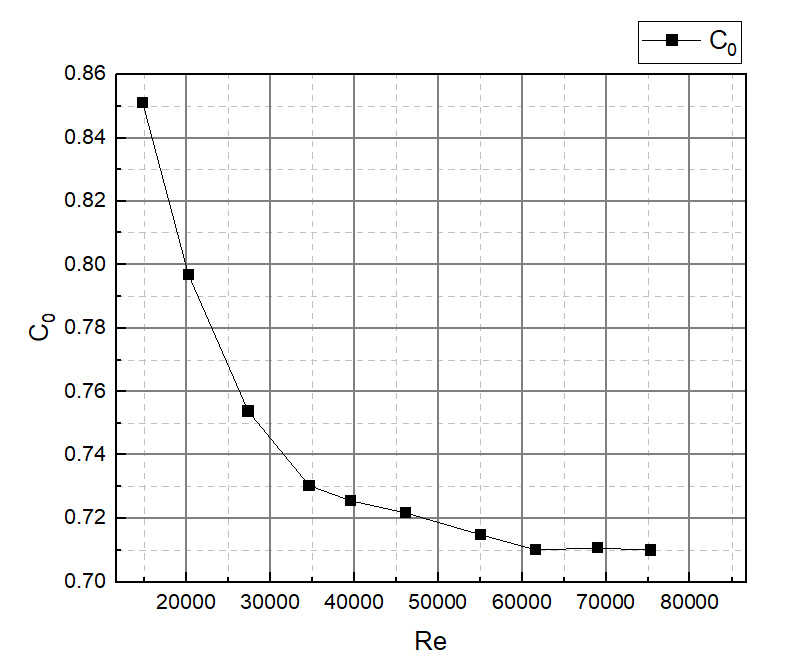
\includegraphics[width=0.7\linewidth]{n.png}
    \caption{孔板流量计孔流系数与雷诺数关系曲线}
    \label{fig:enter-label}
\end{figure}

\subsection{实验结果分析与结论}
\subsubsection{$\lambda$ 与 $Re$ 关系曲线}
三根管的雷诺数与$\lambda$曲线在双对数坐标系下均近似为直线, 其中a管的$\lambda$随雷诺数增加明显下降, 处于阻力一次方区,而bc两管的$\lambda$随雷诺数增加几乎不变, 处于阻力平方区, 此时管道的阻力系数主要由相对粗糙度决定, 而此时c管的阻力系数比b管的更小, 所以可以初步推测c管为铜管而b管为钢管.

b管的关系曲线中出现了一个异常点, 造成这一异常的原因可能是在测量该点的数据时没有等待流动状态稳定就进行读数.

\subsubsection{离心泵特性曲线}
在离心泵的特性曲线中,扬程随流量增加而减少, 轴功率随流量增加而增大, 此离心泵的最高效率点对应的流量约为10.62立方米每时.
\subsubsection{孔板流量计标定}
孔板流量计的孔流系数随雷诺数的增加而减小, 本实验所用的孔板流量计孔流系数大于0.65的近似值. 造成孔流系数变化的原因可能有以下方面:
\begin{enumerate}
    \item 流速越高,流动分离越明显,涡流区域越大,动能损失越严重,这会降低实际通过孔板的流量,使得孔流系数减小。
    \item 在较高雷诺数下,紊流的影响增强,流动更加复杂,尤其是在孔板边缘和下游区域,这种紊流效应会进一步降低孔流系数。
    \item 流体在孔板边缘会形成边界层,随着流速的增加,边界层内的速度梯度增大,流体的动能损失也增大。
\end{enumerate}
        \section{实验思考题}
	1.直管阻力产生的原因是什么?如何测定及计算?

    答:流体在管道内流动时,靠近管壁的流体速度较低,中心区域速度较高,这种速度梯度引起剪切应力,从而导致能量损失。可以通过测量流体通过给定管长的压降来测量.

    2、影响本实验测量准确度的原因有哪些?怎样才能测准数据?
    
    答:主要有管内是否混入气泡,流体流动是否稳定, 以及仪表的精准性等因素. 可以排出管内气泡,改变流速后等待2到3min待流体流动稳定后记录数据。

    3.水平或垂直管中,对相同直径、相同实验条件下所测出的流体的阻力损失是否相同?

    答: 相同, 因为阻力损失实际上是虚拟压差,也即是压差加高差, 所以高度的变化不会影响阻力损失, 如果测量的两点高度不一样那么在计算阻力时需要考虑高度差来算虚拟压差.

    4.根据实验测定数据,如何确定离心泵的工作点?
    
    答:离心泵的工作点就是离心泵特性曲线与管路特性曲线的交点,此时泵给出的能量与管路输送液体所消耗的能量相等。

    5. 电磁流量计测量流量的原理是什么?

    答: 电磁流量计是基于法拉第电磁感应定律工作的流量测量仪表。其核心原理是,当导电流体通过磁场时,会在流体中感应出与流体流速成正比的电动势,通过测量这个电动势来计算流量。

    6. 仔细观察实验装置,提出更多的实验方案,并分析本实验装置存在的问题及改进建议。

    答: 利用高位槽来测阻力损失是比使用离心泵更加简单易行的方法, 本实验装置目前来看比较完善, 如果要改进的话将阀门从手工控制改为电子控制或许是一个方向. 
	
	% 后记(附录)
	%%----------------------------------------------
%	附录Appendix
\appendix{
			\chapter{数据处理所涉及的代码或操作}
   \section{Python 代码}
\begin{lstlisting}[language= Python]
import numpy as np
import scipy as sp

\end{lstlisting}

\section{Origin 操作}
\begin{enumerate}
    \item 打开软件
\end{enumerate}
}
	
	
	% 参考文献
	%\addcontentsline{toc}{chapter}{参考文献}			% 在目录中添加参考文献
	%\bibliographystyle{unsrt}
	%\bibliography{ref/refs}
	
	% 声明
        \addcontentsline{toc}{chapter}{声\hspace{0.8cm}明}
	\section*{声\hspace{0.8cm}明}


%-------------------------------------------------------------------
	本人声明所呈交的实验报告是本人在教师指导下进行的实验工作及取得的实验成果。据我所知,除了文中特别加以标注和致谢的地方外,报告中不包含其他人已经发表或撰写过的成果,也不包含为获得四川大学或其他教育机构的学位或证书而使用过的材料。与我一同工作的同志对本实验所做的任何贡献均已在中作了明确的说明并表示谢意。
	
	本实验报告成果是本人在四川大学修读课程化工原理及仿真实验期间在教师指导下取得的,报告没有所有权归属。任何组织或个人被允许以任何合法目的,在不取得任何许可的情况下使用此报告中的部分或全部内容且需要承担由此引发的全部后果,特此声明。
	
	\vspace{40pt}
	\begin{flushright}
		\begin{tabular}{b{4cm} >{\centering\arraybackslash}b{2.5cm} }
			\songti \zihao{-4} 实验报告作者(签名)& {} \\[-3pt] 
			\cline{2-2} \\ [0.6cm]
                \songti \zihao{-4} 报告指导教师(签名)& {} \\[-3pt] 
			\cline{2-2} \\ [0.6cm]
		\end{tabular}
		
		\today
	\end{flushright}
	
	

	
	
\end{document} 
	
